\Chapter{Aplikacja}\label{chapter:website}
    Rozdział prezentuje praktyczną realizację rozwiązania teoretycznego przedstawionego wcześniej.
    Jego struktura odzwierciedla proces inżynierii oprogramowania, przechodzący od wymagań, przez projekt, aż do implementacji:
    \begin{enumerate}
        \item Specyfikacja wymagań --- formalizuje oczekiwania wobec systemu, dzieląc je na funkcjonalne i niefunkcjonalne, a następnie konkretyzując za pomocą diagramów przypadków użycia i sekwencji.
        \item Projekt systemu --- przedstawia wysokopoziomową architekturę aplikacji, szczegółowy projekt bazy danych oraz makietę interfejsu użytkownika.
        \item Implementacja --- opisuje konkretny stos technologiczny, sposób realizacji poszczególnych komponentów oraz integrację algorytmu z aplikacją webową.
    \end{enumerate}

\section{Specyfikacja wymagań}
    \subsection{Wymagania funkcjonalne}\label{subsection:wymagania_funkcjonalne}
        Aplikacja musi realizować cztery kluczowe grupy funkcjonalności:

        \begin{itemize}
            \item \textbf{Obsługa wielu planów i konfiguracji} --- możliwość pracy z wieloma zestawami zasobów i ograniczeń oraz wieloma planami równolegle.
            \item \textbf{Wprowadzanie danych} --- import plików txt i csv oraz ręczna edycja nauczycieli, klas, przedmiotów, sal, wymagań głównych i bloków przedmiotów.
            \item \textbf{Generowanie planu} --- automatyczne tworzenie planów z możliwością kontroli parametrów algorytmu ewolucyjnego.
            \item \textbf{Przeglądanie planów} --- wizualizacja planów z perspektywy nauczycieli i klas dla wielu wariantów.
        \end{itemize}

    \subsection{Wymagania niefunkcjonalne}
        System musi spełniać następujące wymagania jakościowe:

        \begin{itemize}
            \item \textbf{Wymagania wydajnościowe:}
            \begin{itemize}
                \item Czas generowania kompletnego planu nie powinien przekraczać 10 minut dla typowych przypadków.
                \item Aplikacja musi obsługiwać realistyczne rozmiary danych: do 1000 wymagań głównych, 100 nauczycieli, 50 klas i 100 sal.
                \item Zużycie pamięci operacyjnej nie może przekraczać 8GB podczas generowania planu.
            \end{itemize}
            \item \textbf{Wymagania co do interfejsu:}
            \begin{itemize}
                \item Interfejs powinien być intuicyjny dla użytkowników zaznajomionych z arkuszami kalkulacyjnymi.
                \item Spójność interfejsu we wszystkich modułach aplikacji.
                \item Przejrzystość, minimalizm, wygoda i prostota w użytkowaniu interfejsu.
            \end{itemize}
        \end{itemize}

        Szczegółowa specyfikacja wymagań została przedstawiona na załączonym diagramie przypadków użycia (\ref{fig:diagram_wymagan}).

            \begin{sidewaysfigure}[!p]
                \centering
                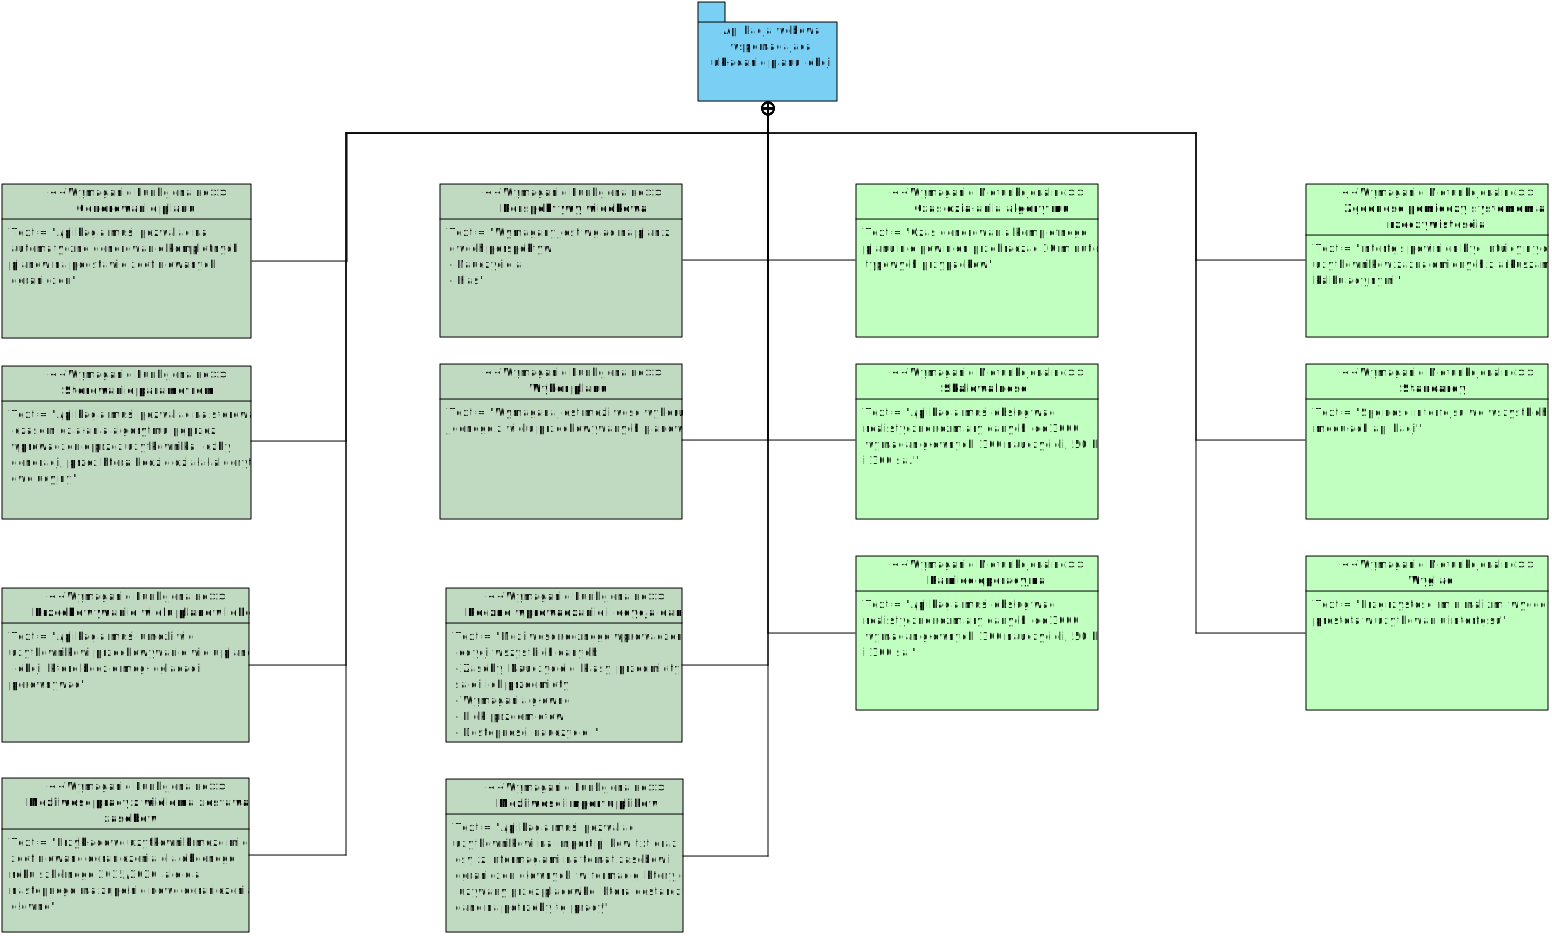
\includegraphics[width=\textwidth,height=\textheight,keepaspectratio]{images/diagramy/Requirement Diagram1.png}
                \caption{Diagram wymagań}\label{fig:diagram_wymagan}
            \end{sidewaysfigure}

    
    % \subsection{Wymagania funkcjonalne}
    %     Najważniejszym aspektem działania aplikacji są funkcjonalności, które ona posiada.
    %     Takie wymagania nazywamy funkcjonalnymi --- definiują one konkretne zachowania i funkcje, które system musi porafić wykonać.

    %     W mojej aplikacji mogę podzielić takie wymagania na 4 grupy:
    %     \begin{itemize}
    %         \item \textbf{Obsługa wielu planów lekcji i konfiguracji:}
    %         \begin{itemize}
    %             \item Tworzenie i przechowywanie wielu planów lekcji.
    %             \item Możliwość pracy z wieloma zestawami zasobów i ograniczeń równolegle.
    %             Przykładowo dla obecnego roku szkolnego mamy zbiór ograniczeń głównych $\mathcal{W}_{2025/2026}$, ale dla następnego jest to juz zupełnie inne zbiór ograniczeń $\mathcal{W}_{2026/2027}$.
    %         \end{itemize}
    %         \item \textbf{Wymagania dotyczące wprowadzania danych:}
    %         \begin{itemize}
    %             \item Import plików \verb|txt| oraz \verb|csv| z zasobami i wymaganiami w formacie używanym przez placówkę, która dostarczyła dane na potrzeby tej pracy.
    %             \item Możliwość ręcznego wprowadzenia i edycji wszystkich typów danych:
    %             \begin{itemize}
    %                 \item Nauczyciele, klasy, przedmioty, sale.
    %                 \item Wymagania główne i bloki przedmiotów.
    %                 \item Dostępności i możliwości sal.
    %             \end{itemize}
    %         \end{itemize}
    %         \item \textbf{Wymagania dotyczące generowania planu lekcji:}
    %         \begin{itemize}
    %             \item Automatyczne generowanie kompletnych planów na podstawie zdefiniowanych ograniczeń.
    %             \item Możliwość sterowania czasem generowania planu poprzez wprowadzanie liczby generacji w algorytmie ewolucyjnym.
    %         \end{itemize}
    %         \item \textbf{Wymagania dotyczące wglądu na utworzone plany:}
    %         \begin{itemize}
    %             \item Wymagany jest wgląd na plan z perspektywy:
    %             \begin{itemize}
    %                 \item Nauczycieli
    %                 \item Klas
    %             \end{itemize}
    %             \item Wymagana jest możliwość wglądu w wiele różnych planów lekcji.
    %         \end{itemize}
    %     \end{itemize}

    % \subsection{Wymagania niefunkcjonalne}
    %     Wymagania niefunkcjonalne określają jakościowe cechy systemu, wpływające na jego użyteczność, wydajność i niezawodność.

    %     Dla rozpatrywanej aplikacji przyjąłem 2 grupy tych wymagań:

    %     \begin{itemize}
    %         \item \textbf{Wymagania wydajnościowe:}
    %         \begin{itemize}
    %             \item Czas generowania kompletnego planu nie powinien przekraczać 10 minut dla typowych przypadków.
    %             \item Aplikacja musi obsługiwać realistyczne rozmiary danych: do 1000 wymagań głównych, 100 nauczycieli, 50 klas i 100 sal.
    %             \item Zużycie pamięci operacyjnej nie może przekraczać 8GB podczas generowania planu.
    %         \end{itemize}
    %         \item \textbf{Wymagania co do interfejsu:}
    %         \begin{itemize}
    %             \item Interfejs powinien być intuicyjny dla użytkowników zaznajomionych z arkuszami kalkulacyjnymi.
    %             \item Spójność interfejsu we wszystkich modułach aplikacji.
    %             \item Przejrzystość, minimalizm, wygoda i prostota w użytkowaniu interfejsu.
    %         \end{itemize}
    %     \end{itemize}

    %     Uwzględnienie zarówno wymagań funkcjonalnych, jak i niefunkcjonalnych pozwala na stworzenie kompletnej aplikacji, która nie tylko realizuje założone funkcje, ale także zapewnia komfortowe i niezawodne środowisko pracy dla docelowych użytkowników.

    \subsection{Przypadki użycia}
        Diagram przypadków użycia pozwala na zwizualizowanie wcześniej omawianych wymagań funkcjonalnych w formie graficznej, ukazując interakcje między użytkownikami a systemem.
        Ułatwia on powiązanie specyfikacji wymagań z projektem architektury, stanowiąc punkt wyjścia do dalszych etapów analizy i implementacji.
        W niniejszej sekcji omawiam kluczowe przypadki użycia zilustrowane na diagramie, obejmujące zarówno generowanie planów lekcji, ich przeglądanie, jak i zarządzanie danymi wejściowymi systemu.

        \begin{figure}[!h]
            \centering
            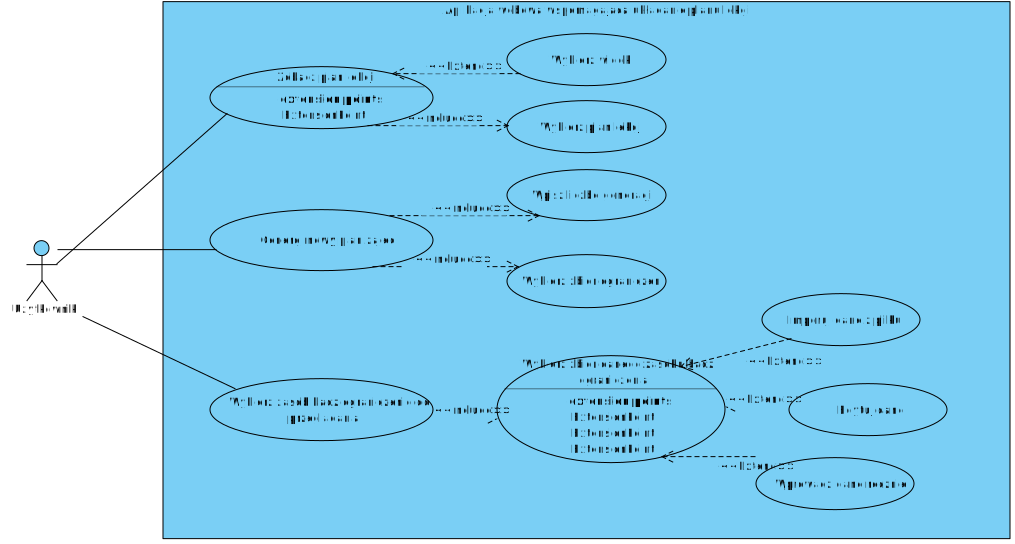
\includegraphics[width=1.0\textwidth]{images/diagramy/Use Case Diagram1.png}
            \caption{Diagram przypadków użycia}\label{fig:usecases}
        \end{figure}

        \begin{table}[h!]
            \centering
            % \setlength{\tabcolsep}{8pt}
            \renewcommand{\arraystretch}{1.4}
            \begin{tabular}{|p{0.25\textwidth}|p{0.70\textwidth}|}
                \hline
                \textbf{Identyfikator} & UC01 \\ \hline
                
                \textbf{Przypadek użycia} & Zobacz plan lekcji \\ \hline
                
                \textbf{Aktor} & Użytkownik \\ \hline
                
                \textbf{Cel} & Sprawdzenie wygenerowanych planów \\ \hline

                \multirow{2}{*}{\textbf{\shortstack[l]{Składowe przypadki\\ użycia}}} 
                & Wybierz widok \\
                & Wybierz plan lekcji \\ \hline

                \multirow{2}{*}{\textbf{Warunki wstępne}} 
                & Wprowadzone zasoby: nauczyciele, sale, klasy, przedmioty \\
                & Przynajmniej jeden wygenerowany plan \\ \hline

                \multirow{1}{*}{\textbf{Stan końcowy}} 
                & Wyświetlony plan lekcji \\ \hline
                
                \multirow{4}{*}{\textbf{Scenariusz}}
                & 1. Użytkownik przechodzi w widok przeglądania planów lekcji \\
                & 2. Użytkownik wybiera plan lekcji \\
                & 3. Użytkownik wybiera widok \\
                & 4. System wyświetla odpowiedni plan lekcji z danej perspektywy \\ \hline
            \end{tabular}
            \caption{Przypadek użycia UC01}
        \end{table}

        \begin{table}[h!]
            \centering
            % \setlength{\tabcolsep}{8pt}
            \renewcommand{\arraystretch}{1.4}
            \begin{tabular}{|p{0.25\textwidth}|p{0.70\textwidth}|}
                \hline
                \textbf{Identyfikator} & UC02 \\ \hline
                
                \textbf{Przypadek użycia} & Wybierz widok \\ \hline
                
                \textbf{Aktor} & Użytkownik \\ \hline
                
                \textbf{Cel} & Wybranie perspektywy oglądania planu lekcji \\ \hline

                \multirow{2}{*}{\textbf{Warunki wstępne}} 
                & Wprowadzone zasoby: nauczyciele, sale, klasy, przedmioty \\
                & Przynajmniej jeden wygenerowany plan \\ \hline

                \multirow{2}{*}{\textbf{Stan końcowy}} 
                & Wybrany nauczyciel bądź klasa \\
                & Plan wyświetlony z perspektywy wybranej klasy bądź nauczyciela \\ \hline
                
                \multirow{6}{*}{\textbf{Scenariusze}}
                & 1a. Użytkownik rozwija listę dostępnych nauczycieli \\
                & 2a. Użytkownik wybiera konkretnego nauczyciela \\
                & 3a. System wyświetla wybranego nauczyciela \\ \cline{2-2}
                & 1b. Użytkownik rozwija listę dostępnych klas \\
                & 2b. Użytkownik wybiera konkretną klasę \\
                & 3b. System wyświetla wybraną klasę \\ \hline
            \end{tabular}
            \caption{Przypadek użycia UC02}
        \end{table}

        \begin{table}[h!]
            \centering
            % \setlength{\tabcolsep}{8pt}
            \renewcommand{\arraystretch}{1.4}
            \begin{tabular}{|p{0.25\textwidth}|p{0.70\textwidth}|}
                \hline
                \textbf{Identyfikator} & UC03 \\ \hline
                
                \textbf{Przypadek użycia} & Wybierz plan lekcji \\ \hline
                
                \textbf{Aktor} & Użytkownik \\ \hline
                
                \textbf{Cel} & Wybranie planu lekcji do podglądu \\ \hline

                \multirow{2}{*}{\textbf{\shortstack[l]{Składowe przypadki\\ użycia}}} 
                & Wybierz zbiór ograniczeń \\
                & Wybierz liczbę generacji \\ \hline

                \multirow{2}{*}{\textbf{Warunki wstępne}} 
                & Wprowadzone zasoby: nauczyciele, sale, klasy, przedmioty \\
                & Przynajmniej jeden wygenerowany plan \\ \hline

                \multirow{2}{*}{\textbf{Stan końcowy}} 
                & Wybrany plan lekcji \\
                & Możliwość wybrania w systemie widoku \\ \hline
                
                \multirow{4}{*}{\textbf{Scenariusz}}
                & 1. Użytkownik rozwija listę dostępnych planów lekcji \\
                & 2. Użytkownik wybiera konkretnego plan lekcji \\
                & 3. System wyświetla nazwę wybranego planu lekcji \\
                & 4. System umożliwia wybranie widoku \\ \hline
            \end{tabular}
            \caption{Przypadek użycia UC03}
        \end{table}

        \begin{table}[h!]
            \centering
            % \setlength{\tabcolsep}{8pt}
            \renewcommand{\arraystretch}{1.4}
            \begin{tabular}{|p{0.25\textwidth}|p{0.70\textwidth}|}
                \hline
                \textbf{Identyfikator} & UC04 \\ \hline
                
                \textbf{Przypadek użycia} & Generuj nowy plan lekcji \\ \hline
                
                \textbf{Aktor} & Użytkownik \\ \hline
                
                \textbf{Cel} & Wygenerowanie nowego planu lekcji na podstawie wybranych ograniczeń \\ \hline

                \multirow{4}{*}{\textbf{Warunki wstępne}} 
                & Wprowadzone zasoby: nauczyciele, sale, klasy, przedmioty \\
                & Wprowadzone wymagania główne \\
                & Wprowadzone dostępności nauczycieli \\
                & Wprowadzone bloki przedmiotów \\ \hline

                \multirow{1}{*}{\textbf{Stan końcowy}}
                & Wyświetlony komunikat o sukcesie operacji \\ \hline

                \multirow{4}{*}{\textbf{Scenariusz}}
                & 1. Użytkownik wybiera zestaw ograniczeń \\
                & 2. Użytkownik wpisuje liczbę generacji \\
                & 3. Użytkownik wybiera opcję generowania planu \\
                & 4. System generuje plan \\
                & 5. System wysyła powiadomienie o zakończeniu procesu \\ \hline
            \end{tabular}
            \caption{Przypadek użycia UC04}
        \end{table}

        \begin{table}[h!]
            \centering
            % \setlength{\tabcolsep}{8pt}
            \renewcommand{\arraystretch}{1.4}
            \begin{tabular}{|p{0.25\textwidth}|p{0.70\textwidth}|}
                \hline
                \textbf{Identyfikator} & UC05 \\ \hline
                
                \textbf{Przypadek użycia} & Wybierz zbiór ograniczeń \\ \hline
                
                \textbf{Aktor} & Użytkownik \\ \hline
                
                \textbf{Cel} & Wybranie zbioru ograniczeń służącego do wygenerowania nowego planu lekcji \\ \hline

                \multirow{1}{*}{\textbf{Warunki wstępne}} 
                & Przynajmniej jeden istniejący zbiór ograniczeń \\ \hline

                \multirow{1}{*}{\textbf{Stan końcowy}} 
                & Wybrany zestaw ograniczeń \\ \hline
                
                \multirow{3}{*}{\textbf{Scenariusz}}
                & 1. Użytkownik rozwija listę dostępnych zestawów ograniczeń \\
                & 2. Użytkownik wybiera konkretny zestaw ograniczeń \\
                & 3. System wyświetla nazwę wybranego zestawu ograniczeń\\ \hline
            \end{tabular}
            \caption{Przypadek użycia UC05}
        \end{table}

        \begin{table}[h!]
            \centering
            % \setlength{\tabcolsep}{8pt}
            \renewcommand{\arraystretch}{1.4}
            \begin{tabular}{|p{0.25\textwidth}|p{0.70\textwidth}|}
                \hline
                \textbf{Identyfikator} & UC06 \\ \hline
                
                \textbf{Przypadek użycia} & Wpisz liczbę generacji \\ \hline
                
                \textbf{Aktor} & Użytkownik \\ \hline
                
                \textbf{Cel} & Wpisanie liczby generacji służącej do wygenerowania planu lekcji \\ \hline

                \multirow{1}{*}{\textbf{Warunki wstępne}} 
                & Przynajmniej jeden istniejący zbiór ograniczeń \\ \hline

                \multirow{1}{*}{\textbf{Stan końcowy}} 
                & Widoczna wpisana liczba generacji \\
                & Możliwa opcja wygenerowania planu lekcji \\ \hline
                
                \multirow{3}{*}{\textbf{Scenariusz}}
                & 1. Użytkownik wpisuje liczbę generacji \\
                & 2. System wyświetla wpisaną liczbę \\
                & 3. System umożliwia wybranie opcji generowania planu lekcji \\ \hline
            \end{tabular}
            \caption{Przypadek użycia UC06}
        \end{table}

        \begin{table}[h!]
            \centering
            % \setlength{\tabcolsep}{8pt}
            \renewcommand{\arraystretch}{1.4}
            \begin{tabular}{|p{0.25\textwidth}|p{0.70\textwidth}|}
                \hline
                \textbf{Identyfikator} & UC07 \\ \hline
                
                \textbf{Przypadek użycia} & Wybierz zasób bądź ograniczenie do przeglądania \\ \hline
                
                \textbf{Aktor} & Użytkownik \\ \hline
                
                \textbf{Cel} & Wybranie zasoby bądź ograniczenia do przeglądania, edytowania bądź wprowadzania \\ \hline

                \multirow{2}{*}{\textbf{\shortstack[l]{Składowe przypadki\\ użycia}}} 
                & Wybierz zbiór danego zasobu bądź ograniczenia \\
                & Stworzy nowy zbiór danego zasobu bądź ograniczenia \\ \hline

                \multirow{1}{*}{\textbf{Warunki wstępne}} 
                & --- \\ \hline

                \multirow{1}{*}{\textbf{Stan końcowy}} 
                & Widoczny widok zasobu bądź ograniczenia \\ \hline
                
                \multirow{7}{*}{\textbf{Scenariusz}}
                & 1. Użytkownik rozwija listę dostępnych zasobów i ograniczeń \\
                & 2. Użytkownik wybiera jeden z nich \\
                & 3. System wyświetla widok danego zasobu \\
                & 4a. Użytkownik wybiera zbiór danego zasobu bądź ograniczenia \\ \cline{2-2}
                & 4b. Użytkownik tworzy nowy zbiór danego zasobu bądź ograniczenia \\ \cline{2-2}
                & 5a. Użytkownik importuje dane z pliku \\ \cline{2-2} 
                & 5b. Użytkownik edytuje dane \\ \cline{2-2}
                & 5c. Użytkownik wprowadza dane ręcznie \\ \hline
            \end{tabular}
            \caption{Przypadek użycia UC07}
        \end{table}

        \begin{table}[h!]
            \centering
            % \setlength{\tabcolsep}{8pt}
            \renewcommand{\arraystretch}{1.4}
            \begin{tabular}{|p{0.25\textwidth}|p{0.70\textwidth}|}
                \hline
                \textbf{Identyfikator} & UC08 \\ \hline
                
                \textbf{Przypadek użycia} & Wybierz zbiór danego zasobu bądź ograniczenia \\ \hline
                
                \textbf{Aktor} & Użytkownik \\ \hline
                
                \textbf{Cel} & Wybranie zbioru zasobu bądź ograniczenia do wglądu \\ \hline

                \multirow{1}{*}{\textbf{Warunki wstępne}} 
                & Przynajmniej jeden istniejący zbiór zasobu bądź ograniczenia \\ \hline

                \multirow{2}{*}{\textbf{Stan końcowy}} 
                & Widoczna nazwa zbioru \\
                & Widoczny wybrany zbiór zasobów bądź ograniczeń \\ \hline
                
                \multirow{4}{*}{\textbf{Scenariusz}}
                & 1. Użytkownik rozwija listę dostępnych zbiorów \\
                & 2. Użytkownik wybiera konkretny zbiór \\
                & 3. System wyświetla nazwę wybranego zbioru \\
                & 4. System wyświetla dany zapisane w bazie danych \\ \hline
            \end{tabular}
            \caption{Przypadek użycia UC08}
        \end{table}

        \begin{table}[h!]
            \centering
            % \setlength{\tabcolsep}{8pt}
            \renewcommand{\arraystretch}{1.4}
            \begin{tabular}{|p{0.25\textwidth}|p{0.70\textwidth}|}
                \hline
                \textbf{Identyfikator} & UC09 \\ \hline

                \textbf{Przypadek użycia} & Wprowadź ręcznie dane \\ \hline

                \textbf{Aktor} & Użytkownik \\ \hline

                \textbf{Cel} & Ręczne wprowadzenie nowych zasobów bądź ograniczeń \\ \hline

                \multirow{1}{*}{\textbf{Warunki wstępne}} 
                & Przynajmniej jeden istniejący zbiór zasobu bądź ograniczenia \\ \hline

                \multirow{2}{*}{\textbf{Stan końcowy}} 
                & Widoczne nowe ograniczenie/zasób \\
                & Nowe ograniczenie/zasób zapisany w bazie danych \\ \hline

                \multirow{3}{*}{\textbf{Scenariusz}}
                & 1. Użytkownik wybiera opcję dodania nowego zasobu bądź ograniczenia \\
                & 2. Użytkownik wpisuje odpowiednie dane \\
                & 3. Użytkownik zapisuje dane \\
                & 3. System wyświetla powiadomienie o powodzeniu zapisu \\ \hline
            \end{tabular}
            \caption{Przypadek użycia UC09}
        \end{table}

        \begin{table}[h!]
            \centering
            % \setlength{\tabcolsep}{8pt}
            \renewcommand{\arraystretch}{1.4}
            \begin{tabular}{|p{0.25\textwidth}|p{0.70\textwidth}|}
                \hline
                \textbf{Identyfikator} & UC10 \\ \hline

                \textbf{Przypadek użycia} & Edytuj dane \\ \hline

                \textbf{Aktor} & Użytkownik \\ \hline

                \textbf{Cel} & Edytowanie istniejących danych \\ \hline

                \multirow{1}{*}{\textbf{Warunki wstępne}} 
                & Przynajmniej jeden istniejący zbiór zasobu bądź ograniczenia \\ \hline

                \multirow{2}{*}{\textbf{Stan końcowy}} 
                & Widoczne zmiany \\
                & Zmiany zapisane w bazie danych \\ \hline

                \multirow{3}{*}{\textbf{Scenariusz}}
                & 1. Użytkownik edytuje wiersz zasobu bądź ograniczenia \\
                & 2. Użytkownik zapisuje dane \\
                & 3. System wyświetla powiadomienie o powodzeniu zapisu \\ \hline
            \end{tabular}
            \caption{Przypadek użycia UC10}
        \end{table}

        \begin{table}[h!]
            \centering
            % \setlength{\tabcolsep}{8pt}
            \renewcommand{\arraystretch}{1.4}
            \begin{tabular}{|p{0.25\textwidth}|p{0.70\textwidth}|}
                \hline
                \textbf{Identyfikator} & UC11 \\ \hline

                \textbf{Przypadek użycia} & Importuj dane z pliku \\ \hline

                \textbf{Aktor} & Użytkownik \\ \hline

                \textbf{Cel} & Import danych z pliku txt lub csv \\ \hline

                \multirow{2}{*}{\textbf{Warunki wstępne}} 
                & Przynajmniej jeden istniejący zbiór zasobu bądź ograniczenia \\ \cline{2-2}
                & Użytkownik posiada plik we właściwym formacie \\ \hline

                \multirow{2}{*}{\textbf{Stan końcowy}} 
                & Widoczne dane, które były w pliku \\
                & Dane zapisane w bazie danych \\ \hline

                \multirow{7}{*}{\textbf{Scenariusz}}
                & 1a. Użytkownik wybiera opcję wybrania pliku źródłowego  \\
                & 2a. Użytkownik wybiera i zatwierdza wybrany plik źródłowy \\ \cline{2-2}
                & 1b. Użytkownik otwiera eksplorator plików \\
                & 2b. Użytkownik przeciąga i upuszcza wybrany plik źródłowy \\ \cline{2-2}
                & 3. System wyświetla dane w pliku \\
                & 4. Użytkownik zapisuje dane \\
                & 5. System wyświetla powiadomienie o powodzeniu zapisu \\ \hline
            \end{tabular}
            \caption{Przypadek użycia UC11}
        \end{table}

        \begin{table}[h!]
            \centering
            % \setlength{\tabcolsep}{8pt}
            \renewcommand{\arraystretch}{1.4}
            \begin{tabular}{|p{0.25\textwidth}|p{0.70\textwidth}|}
                \hline
                \textbf{Identyfikator} & UC12 \\ \hline

                \textbf{Przypadek użycia} & Stwórz nowy zbiór zasobów bądź ograniczeń \\ \hline

                \textbf{Aktor} & Użytkownik \\ \hline

                \textbf{Cel} & Stworzenie nowego zbioru zasobów bądź ograniczeń \\ \hline

                \multirow{1}{*}{\textbf{Warunki wstępne}} 
                & --- \\ \hline

                \multirow{2}{*}{\textbf{Stan końcowy}} 
                & Wybrany zbiór zasobów bądź ograniczeń \\ 
                & Widoczny nowy zbiór zasobów bądź ograniczeń \\ \hline

                \multirow{5}{*}{\textbf{Scenariusz}}
                & Użytkownik wpisuje nazwę nowego zbioru zasobów bądź ograniczeń \\
                & Użytkownik wybiera opcję stworzenia nowego zbioru zasobów bądź ograniczeń \\
                & System wyświetla powiadomienie o powodzeniu zapisu \\
                & System wybiera nowy zbiór zasobów bądź ograniczeń \\ \hline
            \end{tabular}
            \caption{Przypadek użycia UC12}
        \end{table}
    \clearpage

    \subsection{Diagramy sekwencji}
        Diagramy sekwencji stanowią kolejny element modelowania systemu, ukazując sekwencyjny przepływ komunikatów między obiektami w czasie.
        Pozwalają prześledzić interakcje między obiektami w systemie --- od inicjacji akcji w interfejsie, poprzez przetwarzanie w backendzie, aż do generowania planu przez algorytmy.
        W niniejszej sekcji przedstawiam scenariusze współpracy pomiędzy głównymi komponentami aplikacji: interfejsem, warstwą serwerową oraz algorytmem.

        \subsubsection{Diagram sekwencji generowania planu lekcji}
            Najważniejszym do zaprojektowania jest diagram sekwencji generowania planu lekcji.
            Jego poprawne zaprojektowanie ma istotny wpływ na czas oczekiwania użytkownika, ponieważ nadmiarowa komunikacja między interfejsem a backendem może znacząco wydłużyć proces.
            Diagram przedstawia minimalny, konieczny zestaw komunikatów prowadzących do wywołania algorytmu optymalizacyjnego i zwrócenia użytkownikowi gotowego planu.
            \begin{figure}[H]
                \centering
                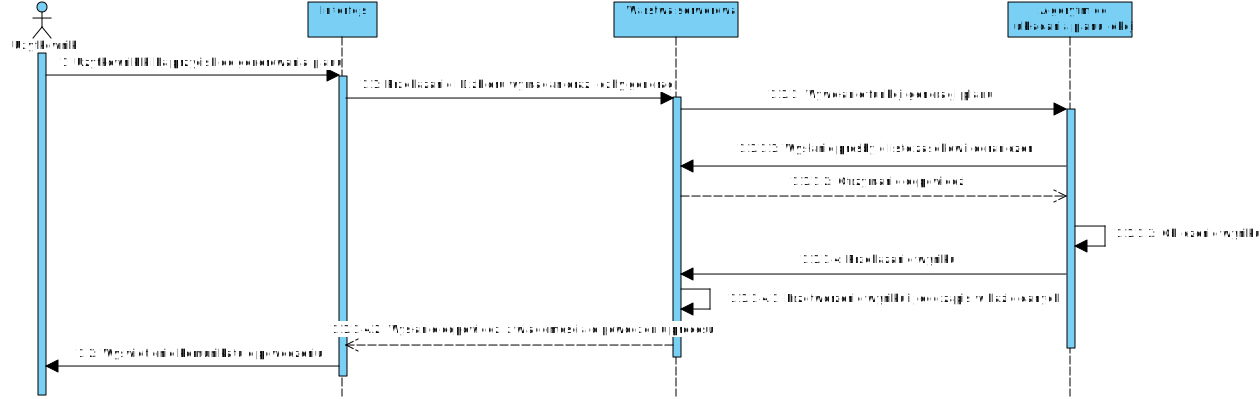
\includegraphics[width=1.0\textwidth]{images/diagramy/Sequence Diagram1.png}
                \caption{Diagram sekwencji generowania planu lekcji}
            \end{figure}
        
        \subsubsection{Diagram sekwencji przeglądania planów lekcji}
            Drugim istotnym scenariuszem jest przeglądanie wygenerowanych planów.
            W tym przypadku kluczowym wymaganiem jest zapewnienie maksymalnej responsywności interfejsu.
            Ciągłe ponawianie zapytań GET przy każdej zmianie widoku byłoby nieefektywne i prowadziłoby do zauważalnych opóźnień.
            
            Z tego powodu zastosowałem inne rozwiązanie --- po wybraniu konkretnego planu aplikacja wykonuje jedno większe zapytanie do bazy danych, a następnie cała dalsza filtracja odbywa się po stronie klienta.
            Minimalnie wydłuża to czas pierwszego ładowania, ale zapewnia pełną płynność późniejszej interakcji.
            \begin{figure}[H]
                \centering
                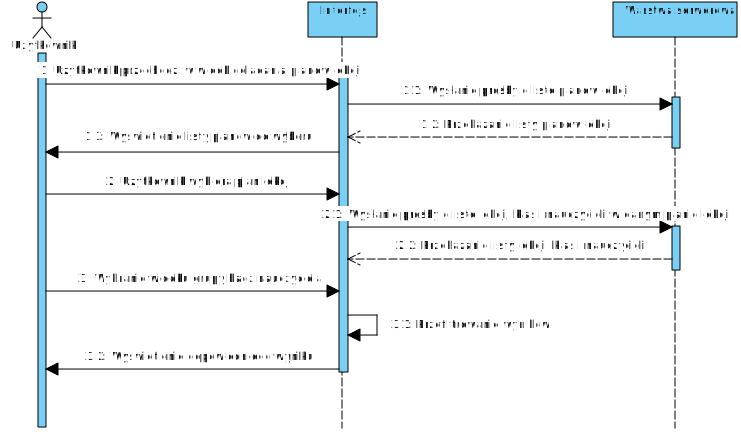
\includegraphics[width=1.0\textwidth]{images/diagramy/Sequence Diagram2.png}
                \caption{Diagram sekwencji dla przypadku użycia oglądania planu lekcji}
            \end{figure}

        \subsubsection{Diagram sekwencji wprowadzania i edycji danych}
            Trzeci scenariusz obejmuje wprowadzanie lub edycję danych, takich jak wymagania główne.
            Kluczowym założeniem było ograniczenie liczby zapytań do serwera przy jednoczesnym zapewnieniu użytkownikowi informacji zwrotnej o powodzeniu operacji.
            \begin{figure}[H]
                \centering
                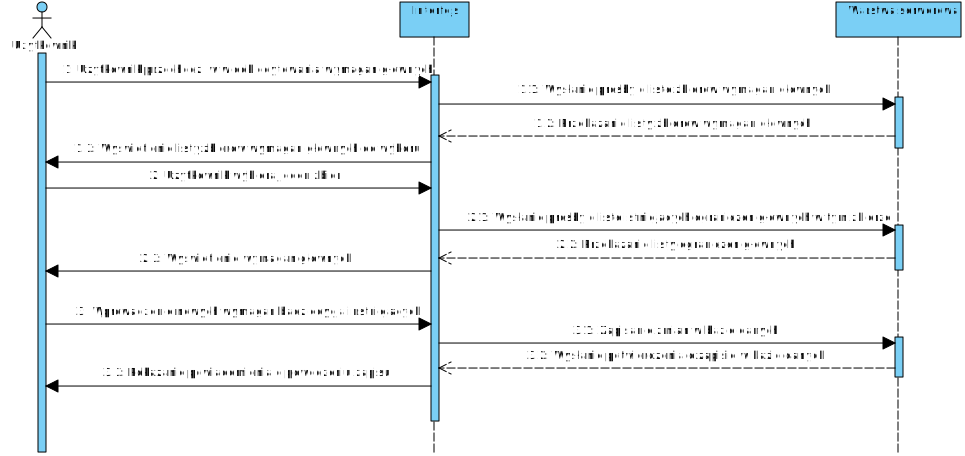
\includegraphics[width=1.0\textwidth]{images/diagramy/Sequence Diagram3.png}
                \caption{Diagram sekwencji edycji bądź wprowadzania wymagań głównych}
            \end{figure}

        \clearpage

\newpage
\section{Projekt}
    \subsection{Architektura systemu}
        Wybór odpowiedniej architektury systemu jest kluczowy dla zapewnienia jego skalowalności, elastyczności i możliwości dalszego rozwoju.
        W celu spełnienia wszystkich wymagań projektowych podzieliłem aplikację na cztery główne komponenty:
        \begin{enumerate}
            \item \textbf{Interfejs użytkownika} (ang. \textit{Graphical User Interface}, GUI) --- odpowiada za komunikację z użytkownikiem, umożliwiając wygodną obsługę systemu bez konieczności znajomości szczegółów działania jego wewnętrznych mechanizmów.
            \item \textbf{Warstwę sewerową} --- umożliwia sprawną integrację wszystkich komponentów poprzez interfejs programowania aplikacji (ang. \textit{Application Programming Interface}, API).
            \item \textbf{Baza danych} --- przechowywuje wszystkie zasoby, ograniczenia oraz plany lekcji w ustrukturyzowany sposób.
            \item \textbf{Moduł optymalizacyjny} --- realizuje algorytmy generowania planów lekcji, przetwarzając dane z bazy i uwzględniając wszystkie wymagania i ograniczenia.
        \end{enumerate}

        \begin{figure}[H]
            \centering
            \begin{tikzpicture}[>=stealth, node distance=2cm]
    
                % Style of blocks
                \tikzstyle{block} = [rectangle, draw, minimum width=3cm, minimum height=1.2cm, align=center]
                \tikzstyle{bigblock} = [rectangle, draw, thick, minimum width=12cm, minimum height=7cm]
            
                % System outline
                \node[bigblock, label=above:{\textbf{System}}] (system) {};
            
                % Blocks inside system
                \node[block] (gui) at ([xshift=-3cm, yshift=1.5cm]system.center) {GUI};
                \node[block] (api) at ([xshift=3cm, yshift=1.5cm]system.center) {API};

                \node[block] (db) at ([xshift=3cm, yshift=-1.5cm]system.center) {Baza danych};
                \node[block] (opt) at ([xshift=-3cm, yshift=-1.5cm]system.center) {Moduł\\optymalizacyjny};

                % User actor
                \node (user) [left=4cm of gui] {
                    \begin{tikzpicture}
                        \draw (0,0) circle (0.3);
                        \draw (0,-0.3) -- (0,-1);
                        \draw (-0.4,-0.6) -- (0.4,-0.6);
                        \draw (0,-1) -- (-0.4,-1.6);
                        \draw (0,-1) -- (0.4,-1.6);
                    \end{tikzpicture}
                };
                \node[below=0.1cm of user] {Użytkownik};

                % Connections
                \draw[<->, very thick, -latex] (user.east) -- (gui.west) node[midway, above]{};
                \draw[<->, very thick, -latex] (gui.east) -- (api.west) node[midway, above]{};
                \draw[<->, very thick, -latex] (api.south) -- (db.north) node[midway, right]{};
                \draw[<->, very thick, -latex] (api.south west) -- (opt.north east) node[midway, above]{};
            
            \end{tikzpicture}
            \caption{Architektura aplikacji}
        \end{figure}

        Taki podział umożliwia niezależny rozwój każdego z komponentów, ułatwia testowanie i utrzymanie systemu, a także pozwala na łatwe skalowanie oraz integrację dodatkowych funkcjonalności w przyszłości.

    \subsection{Projekt struktury bazy danych}\label{subsection:projekt_bazy_danych}
        Projekt bazy danych stanowi kluczowy element architektury aplikacji.
        Jego celem jest umożliwienie wielokrotnego wykorzystania zasobów szkolnych przy jednoczesnej obsłudze zmieniających się wymagań w kolejnych generacjach planów lekcji.

        Aby zapewnić elastyczność, zastosowałem mechanizm zbiorów zasobów oraz zbiorów wymagań, dzięki czemu każdy wygenerowany plan odwołuje się do spójnej konfiguracji danych.

        Poniżej opisałem strukturę bazy danych, dzieląc ją na cztery grupy tabel:
        tabele podstawowe, tabele wymagań, tabele agregujące, oraz tabele wyników.

        \subsubsection{Tabele podstawowe}
            Tabele podstawowe definiują fundamentalne zasoby szkoły, stanowiąc punkt odniesienia dla całego systemu:
            \begin{table}[H]
                \centering
                \begin{tabular}{|r|l|}
                    \hline
                    \textbf{Tabela} & \textbf{Relacja} \\
                    \hline
                    \texttt{subject} & \\
                    \texttt{student\_group} & \\
                    \texttt{teacher} & M:N do \texttt{subject} \\
                    \texttt{room} & M:N do \texttt{subject} \\
                    \hline
                \end{tabular}
                \caption{Tabele podstawowe zasobów szkolnych}
            \end{table}

            \noindent
            gdzie:
            \begin{itemize}
                \item \texttt{subject} przychowuje informacje o przedmiotach.
                \item \texttt{student\_group} przechowuje informacje o klasach.
                \item \texttt{teacher} przechowuje informacje o nauczycielach.
                \begin{itemize}
                    \item Relacja M:N z nauczycielami określa jakich przedmiotów może uczyć dany nauczyciel.
                \end{itemize}
                \item \texttt{room} przechowuje informacje o salach.
                \begin{itemize}
                    \item Relacja M:N z przedmiotami określa jakie przedmioty mogą być prowadzone w danej sali.
                \end{itemize}
            \end{itemize}

            \begin{figure}[H]
                \centering
                \includegraphics[width=0.5\textwidth]{images/diagramy/diagram_db_podstawowe.png}
                \caption{Diagram tabel podstawowych w bazie danych}
            \end{figure}

        \subsubsection{Tabele wymagań}
            Tabele wymagań definiują, co dokładnie należy umieścić w planie lekcji.
            W przeciwieństwie do tabel zasobów nie opisują one tego, co istnieje w szkole, lecz to, jakie lekcji muszą zostać wygenerowane.

            \begin{table}[H]
                \centering
                \begin{tabular}{|r|l|}
                    \hline
                    \textbf{Tabela} & \textbf{Relacje} \\
                    \hline
                    \texttt{requirement} & N:1 z \texttt{teacher}, \texttt{student\_group}, \texttt{subject} \\
                    \texttt{subject\_block} & M:N z \texttt{subject}, M:N z \texttt{student\_group} \\
                    \texttt{teacher\_availability} & N:1 z \texttt{teacher} \\
                    \hline
                \end{tabular}
                \caption{Tabele definiujące wymagania i ograniczenia}
            \end{table}

            \noindent
            gdzie:
            \begin{itemize}
                \item \texttt{requirement} każdy rekord opisuje jedno wymaganie główne.
                \begin{itemize}
                    \item Zawiera klucze obce do tabel przedmiotów, klas, nauczycieli.
                \end{itemize}
                \item \texttt{subject\_block} przechowuje informacje na temat bloków przedmiotów.
                \begin{itemize}
                    \item Relacja M:N z przedmiotami określa jakie przedmioty powinny być w bloku lekcyjnym.
                    \item Relacja M:N z klasami określa jakie klasy powinny być w bloku lekcyjnym.
                \end{itemize}
                \item \texttt{teacher\_availability} przechowuje dostępności nauczycieli. Każdy rekord dotyczy innego nauczyciela.
                \begin{itemize}
                    \item Zawiera klucz obcy do tabeli nauczycieli.
                \end{itemize}
            \end{itemize}

            \begin{figure}[H]
                \centering
                \includegraphics[width=0.8\textwidth]{images/diagramy/diagram_db_wymagan.png}
                \caption{Diagram tabel podstawowych i wymagań w bazie danych}
            \end{figure}

        \subsubsection{Zbiory danych}
            Mechanizm zbiorów umożliwia grupowanie zasobów i wymagań dla różnych kontekstów:

            \begin{table}[H]
                \centering
                \begin{tabular}{|r|l|}
                    \hline
                    \textbf{Tabela} & \textbf{Relacja} \\
                    \hline
                    \texttt{subject\_pool} & M:N z subject \\
                    \texttt{student\_group\_pool} & 1:N z student\_group \\
                    \texttt{teacher\_pool} & M:N z teacher \\
                    \texttt{room\_pool} & 1:N z room \\
                    \hline
                \end{tabular}
                \caption{Tabele zbiorów zasobów}
            \end{table}

            Dla nauczycieli i przedmiotów zastosowałem relację wiele-do-wielu, ponieważ zasoby te charakteryzują się względną stabilnością pomiędzy latami szkolnymi --- większość nauczycieli i przedmiotów pozostaje niezmienna, a jedynie dodawane są nowe rekordy dla nowo zatrudnionych pedagogów lub wprowadzanych przedmiotów.

            W przypadku sal przyjęto relację jeden-do-wielu, co wynika z całkowitej niezmienności tej puli zasobów pomiędzy okresami szkolnymi.
            Natomiast dla klas zastosowałem relację jeden-do-wielu, odzwierciedlającą coroczną całkowitą wymianę składu grup uczniowskich --- klasy z poprzedniego roku nie są ponownie wykorzystywane w kolejnych okresach, co eliminuje potrzebę stosowania relacji wiele-do-wielu.

            Szczególną rolę pełni tabela \texttt{requirement\_set} (zbiór wymagań głównych), ponieważ agreguje wszystkie inne zasoby oraz ogarniczenia.

            \begin{table}[H]
                \centering
                \begin{tabular}{|r|l|}
                    \hline
                    \textbf{Tabela} & \textbf{Relacja} \\
                    \hline
                    \multirow{2}{*}{\texttt{requirement\_set}} & 1:N z \texttt{requirement}, \texttt{teacher\_availability}, \texttt{subject\_block} \\
                    & N:1 z \texttt{subject\_pool}, \texttt{student\_group\_pool}, \texttt{teacher\_pool}, \texttt{room\_pool} \\
                    \hline
                \end{tabular}
                \caption{Tabela requirement\_set}
            \end{table} 

            \noindent
            gdzie:
            \begin{itemize}
                \item \texttt{requirement\_set} każdy rekord opisuje jedno wymaganie główne.
                \begin{itemize}
                    \item Posiada relację 1:N z tabelą \texttt{requirement}, \texttt{teacher\_availability} oraz \texttt{subject\_block}. \\
                    \item Zawiera klucze obce do tabel \texttt{subject\_pool}, \texttt{student\_group\_pool}, \texttt{teacher\_pool} oraz \texttt{room\_pool}.
                \end{itemize}
            \end{itemize}

            Ta struktura umożliwia generowanie kompletnego planu lekcji na podstawie pojedynczego rekordu zbioru wymagań.

            Zaprezentowany model bazy danych zapewnia elastyczność niezbędną do obsługi zmieniających się wymagań szkolnych poprzez mechanizm zbiorów. Struktura umożliwia wielokrotne wykorzystanie zasobów pomiędzy różnymi konfiguracjami planów, zachowując przy tym prostotę i wydajność.

        \subsubsection{Tabele wyników}
            Tabele przechowujące wygenerowane plany lekcji i ich przypisania:

            \begin{table}[H]
                \centering
                \begin{tabular}{|l|l|}
                    \hline
                    \textbf{Tabela} & \textbf{Relacje} \\
                    \hline
                    \texttt{plan} & N:1 z requirement\_set \\
                    \texttt{lesson} & N:1 z teacher, subject, room, student\_group, plan \\
                    \hline
                \end{tabular}
                \caption{Tabele przechowujące wygenerowane plany lekcji}
            \end{table}

            \noindent
            gdzie:
            \begin{itemize}
                \item \texttt{plan} przychowuje plany lekcji dla konkretnego zbioru wymagań (klucz obcy do odpowiedniej tabeli).
                \item \texttt{lesson} przechowuje przypisania. Posiada klucz obcy do wszystkich zasobów oraz planu lekcji.
            \end{itemize}

        \begin{figure}[p]
            \centering
            \includegraphics[width=1.0\textwidth]{images/diagramy/diagram_db_2.png}
            \caption{Diagram pełnego projektu bazy danych}
        \end{figure}

        \begin{table}[p]
            \centering
            \begin{tabular}{|p{0.27\textwidth}|p{0.2\textwidth}|p{0.45\textwidth}|}
                \hline
                \textbf{Tabela} & \textbf{Kolumna} & \textbf{Opis} \\
                \hline
                \multirow{3}{*}{\texttt{student\_group}} & \texttt{id} & Unikalny identyfikator klasy \\
                & \texttt{pool\_id} & Klucz obcy do zbioru klas \\
                & \texttt{name} & Nazwa klasy (,,IIIA'') \\
                & \texttt{desc} & Opis klasy (opcjonalny) \\
                \hline
                \multirow{3}{*}{\texttt{room}} & \texttt{id} & Unikalny identyfikator sali \\
                & \texttt{pool\_id} & Klucz obcy do zbioru sal \\
                & \texttt{name} & Nazwa sali (,,Sala 101'') \\
                \hline
                \multirow{1}{*}{\texttt{subject}} & \texttt{id} & Unikalny identyfikator przedmiotu \\
                & \texttt{name} & Nazwa przedmiotu (,,Matematyka'') \\
                \hline
                \multirow{2}{*}{\texttt{teacher}} & \texttt{id} & Unikalny identyfikator nauczyciela \\
                & \texttt{name} & Imię i/lub nazwisko nauczyciela \\
                \hline
                \multirow{6}{*}{\texttt{requirement\_set}} & \texttt{id} & Unikalny identyfikator zbioru wymagań \\
                & \texttt{teacher\_pool\_id} & Klucz obcy do zbioru nauczycieli \\
                & \texttt{room\_pool\_id} & Klucz obcy do zbioru sal \\
                & \texttt{group\_pool\_id} & Klucz obcy do zbioru klas \\
                & \texttt{subject\_pool\_id} & Klucz obcy do zbioru przedmiotów \\
                & \texttt{name} & Nazwa zbioru wymagań \\
                \hline
                \multirow{4}{*}{\texttt{subject\_block}} & \texttt{id} & Unikalny identyfikator bloku przedmiotów \\
                & \texttt{req\_set\_id} & Klucz obcy do zbioru wymagań \\
                & \texttt{numbers} & Konfiguracja liczby godzin (JSON) \\
                & \texttt{power\_block} & Flaga bloku agregującego \\
                & \texttt{max\_number} & Maksymalna liczba bloków tygodniowo \\
                \hline
                \multirow{3}{*}{\texttt{requirement}} & \texttt{id} & Unikalny identyfikator wymagania \\
                & \texttt{req\_set\_id} & Klucz obcy do zbioru wymagań \\
                & \texttt{teacher\_id} & Klucz obcy do nauczyciela \\
                & \texttt{group\_id} & Klucz obcy do klasy \\
                & \texttt{subject\_id} & Klucz obcy do przedmiotu \\
                & \texttt{hours} & Liczba wymaganych godzin tygodniowo \\
                \hline
                \multirow{3}{*}{\texttt{teacher\_availability}} & \texttt{id} & Unikalny identyfikator dostępności \\
                & \texttt{teacher\_id} & Klucz obcy do nauczyciela \\
                & \texttt{req\_set\_id} & Klucz obcy do zbioru wymagań \\
                & \texttt{availability} & Macierz dostępności (JSON) \\
                \hline
                \multirow{3}{*}{\texttt{plan}} & \texttt{id} & Unikalny identyfikator planu \\
                & \texttt{req\_set\_id} & Klucz obcy do zbioru wymagań \\
                & \texttt{name} & Nazwa planu lekcji \\
                \hline
                \multirow{7}{*}{\texttt{lesson}} & \texttt{id} & Unikalny identyfikator lekcji \\
                & \texttt{plan\_id} & Klucz obcy do planu \\
                & \texttt{teacher\_id} & Klucz obcy do nauczyciela \\
                & \texttt{subject\_id} & Klucz obcy do przedmiotu \\
                & \texttt{room\_id} & Klucz obcy do sali \\
                & \texttt{student\_group\_id} & Klucz obcy do klasy \\
                & \texttt{day} & Dzień tygodnia \\
                & \texttt{hour} & Slot czasowy \\
                \hline
            \end{tabular}
            \caption{Struktura wszystkich tabel w bazie danych}
        \end{table}
    \clearpage

    \subsection{Projekt interfejsu}
        Projekt interfejsu użytkownika opracowałem z uwzględnieniem wymagań funkcjonalnych.
        Architektura nawigacji opiera się na logicznym przepływie pracy charakterystycznym dla procesu układania planu lekcji, zapewniając intuicyjne środowisko dla użytkowników zaznajomionych z arkuszami kalkulacyjnymi.

        \subsubsection{Nawigacja}
            System nawigacji został zaprojektowany jako hierarchiczny, z głównym menu umożliwiającym dostęp do wszystkich kluczowych funkcjonalności.
            Nawigacja górnego poziomu obejmuje przejście między głównymi modułami aplikacji, podczas gdy niższe poziomy zapewniają dostęp do szczegółowych funkcji w obrębie modułu wprowadzania danych.

        \subsubsection{Strona główna}
            Strona główna pełni funkcję centralnego hubu aplikacji. 
            Umożliwia bezpośrednie przejście do trzech kluczowych sekcji: 
            \begin{enumerate}
                \item podglądu istniejących planów lekcji,
                \item wprowadzania i edycji ograniczeń głównych,
                \item modułu generowania nowych planów.
            \end{enumerate}
            
        \subsubsection{Podgląd planów lekcji}
            Strona podglądu planu lekcji umożliwia przeglądanie wielu wariantów planów, co realizuje wymaganie co do możliwości przechowywania wielu planów lekcji.
            Realizuje także wymagania dotyczące wieloperspektywicznego wglądu w wygenerowane plany --- umożliwia wgląd z perspektywy:
            \begin{itemize}
                \item nauczycieli --- prezentujący indywidualne plany zajęć każdego pedagoga,
                \item klas --- ukazujący rozkład zajęć dla poszczególnych grup uczniowskich.
            \end{itemize}

        \subsubsection{Moduły wprowadzania danych}
            Aplikacja zawiera kompleksowy zestaw stron do wprowadzania wszystkich typów danych wymaganych do generowania planu:
            \begin{itemize}
                \item \textbf{Strony zasobów} umożliwiają zarządzanie czterema fundamentalnymi zasobami: przedmiotami, nauczycielami, klasami oraz salami.
                Interfejs powinien zapewniać możliwość ręcznego wprowadzania, edycji i usuwania rekordów, a także importu danych z plików tekstowych w ustalonych formatach.
                \item \textbf{Strona ograniczeń głównych} dedykowana jest definiowaniu wymagań głównych, czyli przypisań godzinowych nauczycieli do klas dla konkretnych przedmiotów.
                Interfejs powinien nawiązywać wyglądem i funkcjonalnością do arkuszy kalkulacyjnych, co ułatwia migrację z dotychczas używanych narzędzi.
                \item \textbf{Strona dostępności nauczycieli} zapewnia graficzny interfejs do określania dni, w których poszczególni nauczyciele są dostępni do prowadzenia zajęć.
                Wykorzystanie intuicyjnych checkboxów z możliwością blokowania i preferowania konkretnych dni.
                \item \textbf{Strona bloków przedmiotów} umożliwia konfigurację bloków przedmiotów, zgodnie z koncepcją przedstawioną w rozdziale~\ref{chapter:algorytm}.
                Interfejs powinien pozwalać na definiowanie składu bloków, klas objętych blokiem, ograniczeń liczbowych oraz flagi agregacji.
            \end{itemize}

        \subsubsection{Moduł generowania planu}
            Strona generowania planu lekcji powinna integrować wszystkie wprowadzone dane i ograniczenia, oferując proste dla użytkownika sterowanie procesem optymalizacji.
            Docelowi użytkownicy nie są osobami zaznajomionymi z technologią, a tym bardziej algorytmami ewolucyjnymi --- nie powinni mieć pełnej kontroli nad wszystkimi parametrami.
            Jedyny parametr, który jest ważny z ich punktu widzenia to liczba generacji algorytmu genetycznego, która jest proporcjonalna do czasu oczekiwania na generację planu.

        \subsubsection{Spójność i ergonomia}
            Wszystkie strony aplikacji powinny utrzymywać spójny schemat wizualny oparty na zasadach minimalizmu i przejrzystości.
            Projekt interfejsu prioritetyzuje wygodę użytkowania poprzez ograniczenie liczby koniecznych kliknięć do wykonania kluczowych operacji oraz zapewnienie natychmiastowego dostępu do najczęściej używanych funkcjonalności.
            
            Wszystkie strony powinny również oferować powiadomienia o wszystkich wykonanych działaniach, tak aby użytkownik wiedział czy jego działania kończą się sukcesem.

\section{Implementacja}
    \subsection{Wybór narzędzi}
        W wyborze stosu technologicznego kierowałem się produktywnością rozwoju aplikacji, skalowalnością rozwiązania oraz integracją z innymi komponentami systemu.

        \subsubsection{Interfejs webowy}
            Decyzja o wykorzystaniu Reacta~\cite{react} jako frameworka frontendowego wynika z kilku kluczowych czynników.
            Po pierwsze, posiadam znaczące doświadczenie w rozwoju aplikacji przy użyciu tej technologii, co pozwoliło na efektywną implementację interfejsu użytkownika.
            Po drugie, React jest jednym z najbardziej popularnych i dojrzałych frameworków frontendowych, co gwarantuje obszerną dokumentację oraz aktywną społeczność wspierającą rozwój.
            Po trzecie, React oferuje responsywne zarządzanie stanem aplikacji, co umożliwia dynamiczną aktualizację widoków planów lekcji bez konieczności przeładowywania strony, zapewniając płynne doświadczenie użytkownika podczas przeglądania planów lekcji.

        \subsubsection{Warstwa serwerowa}
            Wybór Pythona jako głównego języka programowania dla całego systemu był decyzją, podyktowaną koniecznością sprawnej integracji modułu optymalizacyjnego z warstwą aplikacji webowej.
            Implementacja algorytmu generowania planu lekcji w Pythonie umożliwiła wykorzystanie pakietów optymalizacyjnych Google OR-Tools oraz biblioteki NumPy, eliminując potrzebę tworzenia skomplikowanych interfejsów międzyjęzykowych.
            
            Wybór Django~\cite{django} jako frameworka backendowego został dokonany po analizie alternatywnego rozwiązania w Pythonie --- FastAPI.
            Pomimo że FastAPI oferuje wydajność i nowoczesne funkcje, Django zapewnia kompleksowe podejście, które jest lepiej dostosowane do złożonych aplikacji webowych.
            Moje wcześniejsze doświadczenie z Django pozwoliło na efektywną pracę oraz sprawne wykorzystanie technik ORM (ang. \textit{Object-relational mapping}).
            Dodatkowo, skalowalność Django i jego bezpieczeństo zapewniają solidne fundamenty dla aplikacji, która może ewoluować w przyszłości.

        \subsubsection{Baza danych}
            PostgreSQL został wybrany jako system zarządzania bazą danych ze względu na jego wsparcie oraz doskonałą integrację z Django.
            Kluczowym czynnikiem była kompatybilność z biblioteką django-tenants, która umożliwia przyszłą implementację architektury opisanej w jej dokumentacji~\cite{djangotenants}.
            Ta funkcjonalność pozwoli w przyszłości na łatwe dodanie obsługi wielu niezależnych użytkowników lub instytucji w obrębie pojedynczej instancji aplikacji.
            Dodatkowo, wsparcie dla niestandardowych typów danych, między innymi JSON, w PostgreSQL idealnie odpowiada potrzebom przechowywania skomplikowanych struktur danych, takich jak macierze dostępności nauczycieli czy konfiguracje bloków przedmiotów.

        \subsubsection{Moduł optymalizacyjny}
            Moduł optymalizacyjny został zaimplementowany w języku Python, co umożliwiło łatwą integrację z warstwą serwerową oraz szybkie prototypowanie rozwiązań.
            W przypadku algorytmu ewolucyjnego wykorzystałem bibliotekę NumPy, która dzięki zoptymalizowanym operacjom macierzowym znacząco przyspiesza obliczenia i umożliwia efektywne przetwarzanie populacji rozwiązań.

            Algorytm zachłanny oraz algorytm ewolucyjny zostały zaimplementowane od zera, przy użyciu wspomnianej wyżej biblioteki, co pozwoliło na pełną kontrolę nad ich działaniem.
            W trzecim etapie użyłem pakietu Google OR-Tools, który oferuje bogaty zestaw narzędzi do modelowania problemów programowania z ograniczeniami, w tym zmienne interwałowe i ograniczenia typu \verb|NoOverlap|.
            Jego dobra dokumentacja, wysoka wydajność oraz natywna integracja z Pythonem sprawiają, że stanowi on naturalny wybór w tego typu zastosowaniach.

    \subsection{Implementacja bazy danych w Django}
        Technika ORM stosowana w Django oferuje intuicyjny sposób definiowania relacji między modelami.
        
        Relacje wiele-do-jednego są definiowanę klasą \verb|ForeignKey|.
        Relacje wiele-do-wielu implementuje się za pomocą klasy \verb|ManyToManyField|, która automatycznie generuje niezbędne tabele pośredniczące w bazie danych.

        Każda tabela w systemie, z wyjątkiem automatycznie generowanych tabel dla relacji wiele-do-wielu, jest definiowana przez dedykowaną klasę w pliku \verb|models.py|. 
        Na rysunku~\ref{fig:code1} przedstawiłem przykładową implementację modelu reprezentującego sale.

        \subsubsection{Tabela sal}
            \begin{figure}[H]
                \begin{lstlisting}[language=Python]
class Room(models.Model):
    pool = models.ForeignKey(RoomPool, on_delete=models.CASCADE)
    name = models.CharField(max_length=255)
    compatible_subjects = models.ManyToManyField(Subject)
                \end{lstlisting}
                \caption{Fragment kodu służący do definicji tabeli sal}\label{fig:code1}
            \end{figure}

        Analogiczna implementacja dla reszty tabel opisanych w~\ref{subsection:projekt_bazy_danych}.

    \subsection{Implementacja API}
        Warstwa API została zaimplementowana z wykorzystaniem Django REST Framework --- elastycznego zestawu narzędzi do budowy interfejsów REST w Django.
        Znacząco przyspieszyło to proces rozwijania aplikacji poprzez dostarczenie gotowych komponentów do obsługi operacji CRUD, walidacji danych, autentykacji i serializacji.
        Jedną z kluczowych zalet frameworka są automatyczne widoki \verb|ModelViewSet|, które generują kompletny zestaw endpointów dla modelu na podstawie minimalnej konfiguracji, eliminując konieczność ręcznego implementowania rutynowych operacji.
        Takie widoki są również modyfikowalne, co pozwala na uwzględnienie niestandardowych przypadków, takich jak tworzenie wielu wymagań głównych na raz w celu poprawienia wydajności, z relatywną łatwością.

        \begin{figure}[H]
            \centering
            \includegraphics[width=1.0\textwidth]{images/django_api_overview.png}
            \caption{Automatycznie wygenerowana lista endpointów stworzonych przy użyciu \mbox{ModelViewSet}}\label{fig:api_default_router}
        \end{figure}

        Na rysunku~\ref{fig:code2} przedstawiłem przykładową implementację endpointów dotyczących tabeli \verb|room_pool| używając klast \verb|ModelViewSet|.
        \begin{figure}[H]
            \begin{lstlisting}[language=Python]
class RoomPoolSerializer(serializers.ModelSerializer):
    class Meta:
        model = RoomPool
        fields = ["id", "name"]

class RoomPoolViewSet(ModelViewSet):
    queryset = RoomPool.objects.all()
    serializer_class = RoomPoolSerializer
            \end{lstlisting}
            \caption{Fragment kodu służący do implementacji endpointów dla zbioru sal}\label{fig:code2}
        \end{figure}

    \subsection{Implementacja interfejsu webowego}
        Komponentowa architektura Reacta pozwoliła na zbudowanie modularnego interfejsu, gdzie poszczególne widoki (takie jak edycja wymagań, konfiguracja zasobów czy podgląd planów) zostały wydzielone jako niezależne komponenty, które w połączeniu z komponentem nawigacji tworzą konkretne strony.
        Połączenie z backendem realizowane jest poprzez zdefiniowane powyżej API, zapewniając płynną komunikację między warstwą interfejsu a warstwą serwerową.

        \subsubsection{Nawigacja}
            Nawigacja przedstawiona na rysunku~\ref{fig:nawigacja} składa się z trzech elementów:
            \begin{itemize}
                \item Po lewej stronie znajduje się nazwa aplikacji. 
                \item Na środku wyświetlana jest aktualna nazwa podstrony, co pomaga użytkownikowi szybko zorientować się w kontekście.
                \item Po prawej dostępne są główne sekcje aplikacji, w tym rozwijane menu ,,Upload Requirements'', umożliwiające przejście do konkretnych modułów wprowadzania danych.
            \end{itemize}

            \begin{figure}[H]
                \centering
                \includegraphics[width=0.9\textwidth]{images/strona/nawigacja.png}
                \caption{Nawigacja interfejsu webowego}\label{fig:nawigacja}
            \end{figure}

        \subsubsection{Strona główna}
            Strona główna przedstawiona na rysunku~\ref{fig:glowna} zapewnia szybki dostęp do kluczowych funkcji aplikacji: przeglądania istniejących planów lekcji, generowania nowych oraz wprowadzania wymagań głównych.
            
            \begin{figure}[H]
                \centering
                \includegraphics[width=0.9\textwidth]{images/strona/strona_glowna.png}
                \caption{Strona główna interfejsu webowego}\label{fig:glowna}
            \end{figure}
            
            \subsubsection{Podgląd planów lekcji}
                Widok planów lekcji można przeglądać zarówno z perspektywy klas, jak i nauczycieli.
                W widoku klas każda lekcja prezentowana jest wraz z przypisanym nauczycielem, natomiast w widoku nauczyciela wyświetlane są klasy, z którymi prowadzi zajęcia.

                Implementacja zaprezentowana na rysunku~\ref{fig:plan_nauczyciel} oraz~\ref{fig:plan_klasa} spełnia wymagania funkcjonalne co do przeglądania planów.

                \begin{figure}[H]
                    \centering
                    \includegraphics[width=0.9\textwidth]{images/strona/plan_nauczyciel.png}
                    \caption{Podgląd planu z perspektywy nauczyciela}\label{fig:plan_nauczyciel}
                \end{figure}
                \begin{figure}[H]
                    \centering
                    \includegraphics[width=0.9\textwidth]{images/strona/plan_klasa.png}
                    \caption{Podgląd planu z perspektywy klasy}\label{fig:plan_klasa}
                \end{figure}

        \subsubsection{Widok generowania planów lekcji}
            Widok umożliwia użytkownikowi określenie liczby generacji, jakie algorytm powinien wykonać podczas tworzenia planu lekcji.
            Dzięki temu można dostosować czas działania i potencjalną jakość rozwiązania do bieżących potrzeb.

            Implementacja zaprezentowana na rysunku~\ref{fig:plan_generowanie} spełnia wymagania funkcjonalne co do generowania planu lekcji.

            \begin{figure}[H]
                \centering
                \includegraphics[width=0.9\textwidth]{images/strona/generowanie.png}
                \caption{Widok generowania planu lekcji}\label{fig:plan_generowanie}
            \end{figure}

        \subsubsection{Widoki wprowadzania zasobów}
            Widoki wprowadzania zasobów pozwalają na tworzenie, i wybieranie ich zbiorów.
            Implementacje przedstawione na rysunkach~\ref{fig:add_subject},~\ref{fig:add_teacher},~\ref{fig:add_room},~\ref{fig:add_class} spełniają wymagania funkcjonalne co do dodawania zasobów.

            \begin{figure}[H]
                \centering
                \includegraphics[width=0.9\textwidth]{images/strona/przedmioty.png}
                \caption{Widok dodawania przedmiotów}\label{fig:add_subject}
            \end{figure}
            \begin{figure}[H]
                \centering
                \includegraphics[width=0.9\textwidth]{images/strona/nauczyciele.png}
                \caption{Widok dodawania nauczycieli}\label{fig:add_teacher}
            \end{figure}
            \begin{figure}[H]
                \centering
                \includegraphics[width=0.9\textwidth]{images/strona/sale.png}
                \caption{Widok dodawania sal}\label{fig:add_room}
            \end{figure}
            \begin{figure}[H]
                \centering
                \includegraphics[width=0.9\textwidth]{images/strona/klasy.png}
                \caption{Widok dodawania klas}\label{fig:add_class}
            \end{figure}

        \subsubsection{Widoki wprowadzania wymagań}
            Widok wprowadzania wymagań głównych przedstawiony na rysunku~\ref{fig:wprowadzanie_glowne}, który przypomina arkusz kalkulacyjny pokazany na rysunku~\ref{fig:excel_wymagania}, co spełnia wymagania niefunkcjonalne.
            Górny wiersz przewija się razem ze stroną ułatwiając nawikację i wpisywanie wymagań.
            Podobnie jak widoki wprowadzania zasobów pozwala na wybranie zbioru wymagań głównych, co realizuje wymagania funkcjonalne co do pracy z wieloma zestawami zasobów.

            Na podobnej zasadzie działają widoki wprowadzania dostępności nauczycieli i bloków przedmiotów przedstawione odpowiednio na rysunkach~\ref{fig:dostepnosc_nauczycieli} i~\ref{fig:wprowadzenie_blokow}.

            \begin{figure}[H]
                \centering
                \includegraphics[width=0.9\textwidth]{images/strona/wymagania_glowne_1.png}
                \vspace{1em}
                \includegraphics[width=0.9\textwidth]{images/strona/wymagania_glowne_2.png}
                \caption{Widok dodawania wymagań głównych}\label{fig:wprowadzanie_glowne}
            \end{figure}
            \begin{figure}[H]
                \centering
                \includegraphics[width=0.9\textwidth]{images/strona/dostepnosc.png}
                \caption{Widok wprowadzania dostępności nauczycieli}\label{fig:dostepnosc_nauczycieli}
            \end{figure}
            \begin{figure}[H]
                \centering
                \includegraphics[width=0.9\textwidth]{images/strona/bloki.png}
                \caption{Widok dodawania bloków przedmiotów}\label{fig:wprowadzenie_blokow}
            \end{figure}

    \subsection{Integracja z algorytmem}
        Dzięki adekwatnemu wyborowi technologii, proces integracji modułu optymalizacyjnego z warstwą serwerową został znacząco uproszczony.
        Zaimplementowałem dedykowany endpoint, który przyjmuje żądania typu POST zawierające parametry konfiguracyjne algorytmu, w tym liczbę generacji dla algorytmu ewolucyjnego oraz ID zbioru wymagań.\\
        Proces generowania planu lekcji przebiega według następującego schematu:
        \begin{enumerate}
            \item Pobranie i walidacja danych wejściowych z żądania.
            \item Wczytanie odpowiedniego zestawu ograniczeń i wymagań z bazy danych.
            \item Uruchomienie trójetapowego algorytmu optymalizacyjnego z przekazanymi parametrami.
            \item Transformacja wyników algorytmu do przypisań lekcyjnych.
            \item Utworzenie nowego rekordu planu lekcji w bazie danych.
            \item Zapisanie wygenerowanych przypisań (lekcji) w powiązaniu z utworzonym planem.
            \item Zwrócenie odpowiedzi zawierającej status operacji.
        \end{enumerate}


        % Dzięki adekwatnemu wyborze technologii proces integracji modułu optymalizacyjnego z warstwą serwerową był prosty.
        % Stworzyłem endpoint do którego interfejs webowy może wysyłać zapytanie typu POST z wartością liczbową mówiącą i liczbie generacji.
        % Cały proces można opisać w następujących krokach:
        % \begin{enumerate}
        %     \item Uruchom algorytm z odpowiednimi ograniczeniami podanymi w zapytaniu
        %     \item Przetwórz wynik algorytmu na przypisania
        %     \item Stwój nowy plan lekcji
        %     \item Zapisz przypisania w stworzonym planie lekcji
        %     \item Zapisz plan lekcji i przypisania (lekcje) w bazie danych
        %     \item Zwróć wiadomość o sukcesie bądź ewentualnych błędach
        % \end{enumerate}